\documentclass[11pt,a4paper]{article}

\usepackage[utf8]{inputenc}
\usepackage[T1]{fontenc}
\usepackage[spanish,es-noshorthands,es-tabla]{babel}
\usepackage{lmodern}
\usepackage{microtype}
\usepackage[margin=2.3cm]{geometry}
\usepackage{xcolor}
\usepackage{graphicx}
\usepackage{float}
\usepackage{booktabs}
\usepackage{tabularx}
\usepackage{listings}
\usepackage[most]{tcolorbox}
\usepackage{tikz}
\usetikzlibrary{arrows.meta,positioning,calc}
\usepackage[hidelinks]{hyperref}

\setlength{\parindent}{0pt}
\setlength{\parskip}{0.6em}

% ---------- colores ----------
\definecolor{udpfill}{HTML}{DCFCE7}\definecolor{udpline}{HTML}{166534}
\definecolor{tcpfill}{HTML}{DBEAFE}\definecolor{tcpline}{HTML}{1E40AF}
\definecolor{redfill}{HTML}{FEF3C7}\definecolor{redline}{HTML}{92400E}
\definecolor{errline}{HTML}{991B1B}
\definecolor{gristxt}{HTML}{57606A}
\definecolor{codebg}{HTML}{F6F8FA}

% ---------- caja de la pregunta ----------
\newtcolorbox{pregunta}[1]{enhanced,breakable,colback=tcpfill,colframe=tcpline,
  boxrule=0.6pt,arc=2mm,left=2mm,right=2mm,top=1mm,bottom=1mm,
  fonttitle=\bfseries,title={#1}}

% ---------- código ----------
\lstset{
  basicstyle=\ttfamily\footnotesize,
  backgroundcolor=\color{codebg},
  frame=single, rulecolor=\color{gray!40},
  columns=fullflexible, keepspaces=true,
  breaklines=true, showstringspaces=false,
  commentstyle=\color{gristxt}\itshape,
  keywordstyle=\color{tcpline}\bfseries,
  xleftmargin=2pt, xrightmargin=2pt, aboveskip=0.6em, belowskip=0.6em,
  literate={á}{{\'a}}1 {é}{{\'e}}1 {í}{{\'i}}1 {ó}{{\'o}}1 {ú}{{\'u}}1 {ñ}{{\~n}}1
}
\newcommand{\pipe}{\texttt{|}}
\newcommand{\code}[1]{\texttt{#1}}
\newcommand{\crlf}{\code{\textbackslash r\textbackslash n}}

% ---------- capturas de Wireshark ----------
% \captura{archivo}{ancho}{qué recortar}: si el PNG todavía no está en capturas/,
% se dibuja un recuadro con las instrucciones para sacarlo.
\newcommand{\captura}[3]{%
  \IfFileExists{capturas/#1}%
    {\includegraphics[width=#2\textwidth]{capturas/#1}}%
    {\fbox{\parbox{0.92\textwidth}{\centering\small\color{errline}
      \textbf{Falta la imagen \code{capturas/#1}}\\[0.3em]\color{black}#3}}}}

\begin{document}

% ======================================================================
\begin{center}
  {\small UdeSA -- I310 Redes y Comunicación -- 2026s2}\\[0.8em]
  {\LARGE\bfseries TP D: Desarrollo de aplicaciones distribuidas\\[0.2em] con BSD sockets}\\[0.8em]
  {\large Respuestas a las preguntas y entregables}\\[0.8em]
  {\bfseries Grupo 5 (\code{grupo05})}\\[0.3em]
  Luis Embon Strizzi \quad·\quad Alan Yeger \quad·\quad Franco Kirchheimer
\end{center}

\tableofcontents

% ======================================================================
\section{Ejecución de los desafíos}

Nuestro cliente resuelve los dos desafíos. Primero obtiene la IP pública con un pedido HTTP escrito a mano sobre TCP a \code{api.ipify.org}, y con ella se autentica por UDP ante el servidor de la cátedra mediante una firma MD5 que implementamos siguiendo el RFC~1321. Una vez que verifica la respuesta firmada, se conecta por TCP al puerto que le asignaron, separa las PDUs que llegan por ese flujo de bytes y, a medida que las completa, las valida y las reenvía firmadas por UDP. Toda la ejecución quedó registrada en \code{TP\_D\_captura2.pcapng}, tomada con el filtro \code{ip.addr == 167.114.129.206 || tcp.port == 80}, es decir, el tráfico con el servidor de la cátedra más la consulta HTTP a ipify.

\subsection{Desafío 1: autenticación}

La Figura~\ref{fig:auth} muestra el intercambio completo. El pedido (frame~10) sale del puerto efímero 56872 hacia el 20262 con 55 bytes de datos, que corresponden al texto \code{grupo05|190.225.36.143|<firma>}, donde la IP es la pública que nos devolvió ipify, ya que nuestra máquina tiene la dirección privada \code{192.168.1.25}. La respuesta \code{200|Port|30029|<firma>}, de 47 bytes, vuelve 180~ms después al mismo puerto 56872 (frame~12), y apenas 1,2~ms más tarde comienza el \emph{3-way handshake} hacia el puerto asignado (frames 13 a 15). El frame~11 es un ACK tardío de la conexión con ipify, que ya se estaba cerrando. El contenido de ambos datagramas puede leerse en la Figura~\ref{fig:udp}.

\begin{figure}[H]
\centering
\captura{fig1-autenticacion.png}{0.98}{Abrir \code{TP\_D\_captura2.pcapng}, aplicar el filtro de visualización \code{frame.number >= 10 \&\& frame.number <= 15} y seleccionar el frame~12. Recortar la lista de paquetes (frames 10 a 15) junto con el panel de bytes, donde se lee \code{200|Port|30029|\ldots}.}
\caption{Pedido de autenticación (frame 10), respuesta con el puerto (frame 12) y \emph{handshake} hacia el puerto 30029 (frames 13 a 15).}
\label{fig:auth}
\end{figure}

\subsection{Desafío 2: framing y reenvío de PDUs}

El servidor manda diez PDUs por la conexión TCP y las agrupa de distintas maneras en los segmentos, que es precisamente lo que el framing tiene que resolver. En el frame~19 llegan dos PDUs completas dentro de un único segmento de 49 bytes, y nuestro cliente responde con dos reportes UDP consecutivos (frames 21 y 22). En cambio, la cuarta PDU llega partida en tres segmentos de 16, 16 y 5 bytes (frames 23, 25 y 27), y su reporte sale recién en el frame~29, cuando aparece el delimitador \crlf. La Figura~\ref{fig:framing} muestra ambos casos.

\begin{figure}[H]
\centering
\captura{fig2-framing.png}{0.98}{Aplicar el filtro \code{frame.number >= 16 \&\& frame.number <= 31} y recortar la lista de paquetes. Conviene que se vea la columna \emph{Length} (o \emph{TCP segment len}) para mostrar los segmentos de 49, 16, 16 y 5 bytes y los UDP que salen después.}
\caption{Dos PDUs en un segmento (frame 19) seguidas de dos reportes, y una PDU partida en tres segmentos (frames 23, 25 y 27) con un único reporte al final.}
\label{fig:framing}
\end{figure}

El contenido completo del flujo, visto con \emph{Follow TCP Stream}, aparece en la Figura~\ref{fig:stream}. Allí se distinguen las diez PDUs, incluida \code{17x0000000\&Mensaje | invalido}, que no reenviamos porque contiene el carácter \pipe{}, y las que provocan los códigos 408, 406, 407, 409 y 410.

\begin{figure}[H]
\centering
\captura{fig3-tcp-stream.png}{0.85}{Hacer clic derecho sobre cualquier paquete del puerto 30029 (por ejemplo el frame 16), elegir \emph{Follow} $\to$ \emph{TCP Stream} y recortar la ventana con el texto de las diez PDUs.}
\caption{Las diez PDUs que envió el servidor, vistas con \emph{Follow TCP Stream}.}
\label{fig:stream}
\end{figure}

Del lado de UDP, la Figura~\ref{fig:udp} muestra la conversación con el puerto 20262 vista con \emph{Follow UDP Stream}, donde en rojo aparece lo que envía el cliente y en azul lo que responde el servidor. La primera línea es el pedido de autenticación y la segunda la respuesta con el puerto, y a continuación se suceden los nueve reportes, uno por cada PDU sin \pipe{}. Wireshark los muestra pegados porque concatena el contenido de los datagramas, pero cada reporte viajó en un datagrama propio, de modo que sus límites nunca se pierden, a diferencia de lo que ocurre con las PDUs en el flujo TCP. También se observa que, después de la respuesta con el puerto, el servidor no vuelve a enviar nada, es decir, no confirma los reportes.

\begin{figure}[H]
\centering
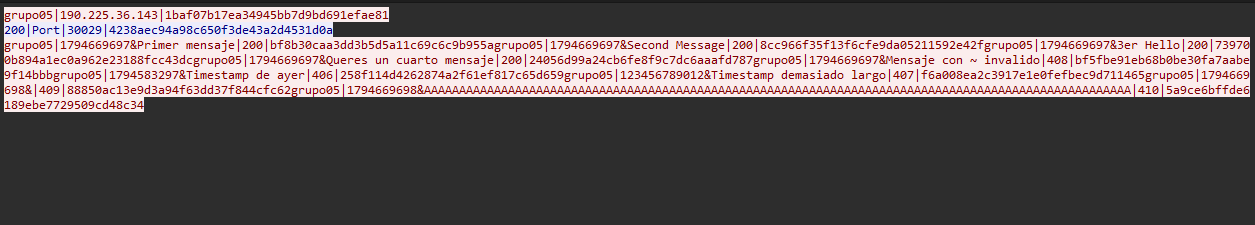
\includegraphics[width=\textwidth]{capturas/fig4-udp-stream.png}
\caption{La conversación UDP con el puerto 20262 (\emph{Follow UDP Stream}): pedido, respuesta con el puerto y los nueve reportes.}
\label{fig:udp}
\end{figure}

Por último, la página de la cátedra confirma el resultado (Figura~\ref{fig:web}). Las PDUs 1 a 4 y 6 a 10 figuran con el código que informamos igual al esperado, mientras que la PDU~5, la que contiene \pipe{}, aparece como N/A porque no debía reenviarse. Esto también confirma una decisión que habíamos tomado ante una ambigüedad del enunciado, que es enviar el campo \code{<PDU>} del reporte sin el \crlf, dado que ese par de bytes es el delimitador y no forma parte del mensaje.

\begin{figure}[H]
\centering
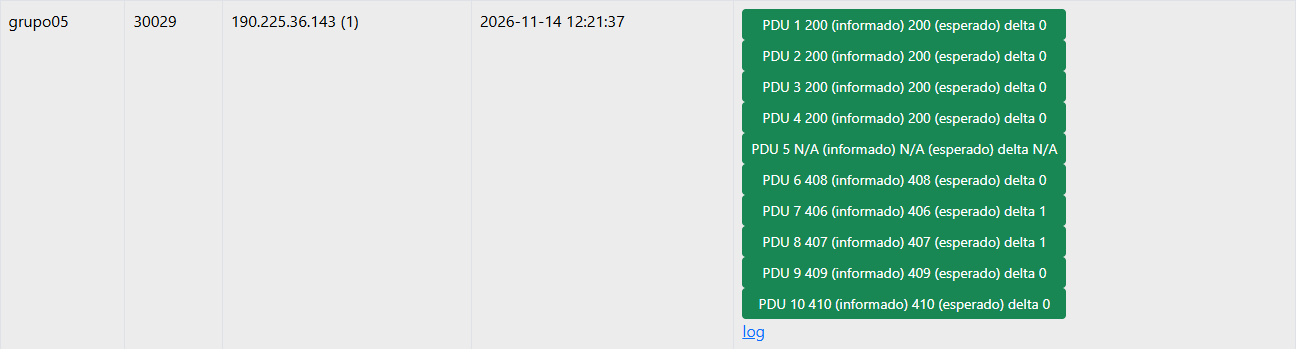
\includegraphics[width=\textwidth]{capturas/web-catedra.png}
\caption{Resultado del grupo 5 en la página de la cátedra: los diez casos, en verde.}
\label{fig:web}
\end{figure}

% ======================================================================
\section{Pregunta 1: reenviar PDUs que contienen 0x7C}

\begin{pregunta}{Pregunta 1}
¿Cómo podría mejorar el protocolo para permitir el reenvío de PDUs por UDP con el carácter prohibido usado para la delimitación 0x7C?
\end{pregunta}

El problema de fondo es que el reporte \code{<USERNAME>|<PDU>|<PARSE\_CODE>|<SIGNATURE>} usa el mismo byte \code{0x7C} para separar sus campos y para transportar datos. Cuando la PDU contiene ese carácter, un receptor que corte en cada \pipe{} ya no puede saber dónde termina un campo y empieza el siguiente, como ocurre con la PDU que envía el servidor:

\begin{lstlisting}
grupo05|17x0000000&Mensaje | invalido|405|<firma>     <- 5 campos en vez de 4
\end{lstlisting}

Por ese motivo nuestro cliente descarta esa PDU antes de firmarla, tal como pide la consigna. Sin embargo, el protocolo podría admitirla de varias maneras.

La mejora más económica ni siquiera cambia el formato del mensaje, sino la forma en que el servidor lo interpreta. Como el usuario solo admite \code{[0-9A-Za-z]}, el código tiene siempre tres dígitos y la firma tiene 32 caracteres hexadecimales, ninguno de esos campos puede contener \pipe{}. Por lo tanto, el servidor puede tomar el usuario hasta el primer separador, la firma después del último y el código entre el penúltimo y el último, de modo que todo lo que queda en el medio es la PDU, tenga los \pipe{} que tenga. La limitación de esta idea es que solo funciona mientras exista un único campo de contenido libre.

Una solución más general, y la que nos parece más robusta, consiste en anteponer la longitud de la PDU, por ejemplo \code{grupo05|29|17x0000000\&Mensaje | invalido|405|<firma>}. El receptor lee el número y toma exactamente esa cantidad de bytes sin mirar su contenido, del mismo modo que lo hacen el campo \emph{Total Length} de IP, el \emph{Length} de UDP o el encabezado \code{Content-Length} de HTTP.

Otra alternativa es el \emph{byte stuffing}, que reemplaza cada \pipe{} de la PDU por una secuencia de escape como \code{\textbackslash|}, tal como hacen HDLC y PPP con su byte de bandera. En ese caso también hay que escapar el propio carácter de escape, porque \code{\textbackslash} (\code{0x5C}) es un carácter válido del mensaje, y el receptor debe deshacer el escape antes de verificar la firma. Finalmente, se podría codificar la PDU en hexadecimal o en base64, cuyos alfabetos no incluyen \pipe{}. Es la opción más simple de implementar, aunque agranda el mensaje: una PDU de 120 bytes pasaría a ocupar 240 en hexadecimal o 160 en base64, lo cual de todos modos entra holgadamente en un datagrama.

En cualquiera de estas variantes conviene que la firma se siga calculando sobre la PDU original, para que el cliente y el servidor firmen exactamente los mismos bytes sin importar cómo se transportaron.

% ======================================================================
\section{Pregunta 2: ¿podría el servidor iniciar la conexión TCP?}

\begin{pregunta}{Pregunta 2}
¿Podría cambiarse el rol de quien inicia la conexión TCP para el segundo desafío? Es decir, ¿podría el servidor iniciar la conexión TCP contra sus computadoras con el programa de Sockets? Argumente su respuesta.
\end{pregunta}

En principio el protocolo podría redefinirse así, pero en las redes desde las que trabajamos los alumnos no funcionaría, y el motivo principal es el NAT. Nuestra computadora tiene la dirección privada \code{192.168.1.25} y sale a Internet con la dirección pública del router, \code{190.225.36.143}; de hecho, el desafío 1 nos obliga a consultar ipify justamente porque esa es la única dirección que el servidor puede ver. Un NAPT traduce cada par (IP privada, puerto) a un par (IP pública, puerto) y crea la entrada correspondiente en su tabla recién cuando sale el primer paquete desde adentro.

\begin{center}
\begin{tikzpicture}[font=\small,
  host/.style={draw,rounded corners=2pt,minimum width=2.6cm,minimum height=1.0cm,align=center},
  >={Stealth[length=2.2mm]}]
  \node[host,fill=tcpfill,draw=tcpline] (c) {cliente\\\code{192.168.1.25}};
  \node[host,fill=redfill,draw=redline,right=3.3cm of c] (n) {router NAT\\\code{190.225.36.143}};
  \node[host,fill=udpfill,draw=udpline,right=3.3cm of n] (s) {servidor\\\code{167.114.129.206}};
  \draw[->,udpline,thick] ($(c.east)+(0,0.30)$) -- node[above,font=\scriptsize]{UDP :56872 $\to$ :20262} ($(n.west)+(0,0.30)$);
  \draw[->,udpline,thick] ($(n.east)+(0,0.30)$) -- node[above,font=\footnotesize]{crea la entrada} ($(s.west)+(0,0.30)$);
  \draw[->,errline,thick] ($(s.west)+(0,-0.30)$) -- node[below,font=\scriptsize]{SYN nuevo $\to$ :???} ($(n.east)+(0,-0.30)$);
  \node[errline,font=\bfseries\large] at ($(n.east)+(0.25,-0.30)$) {$\times$};
  \node[below=0.45cm of n,align=center,font=\footnotesize,text=gristxt]
    {sin entrada en la tabla, el router no sabe\\a qué equipo de la red privada entregarlo y lo descarta};
\end{tikzpicture}
\end{center}

Esto explica por qué el servidor sí puede respondernos por UDP: fuimos nosotros quienes enviamos primero, de modo que el datagrama del frame~10 creó la entrada y la respuesta del frame~12 regresa a través de ella. Por la misma razón nuestra función \code{enviar\_pedido} devuelve el socket en lugar de cerrarlo, y los nueve reportes salen por ese mismo socket. En cambio, un SYN iniciado por el servidor llegaría al router como un paquete no solicitado, sin ninguna entrada que lo asocie a un equipo interno, y sería descartado. Tampoco serviría la entrada creada por el tráfico UDP, ya que la tabla distingue protocolo y puertos. Se trata del mismo problema que vimos con FTP en modo activo, donde es el servidor quien abre la conexión de datos hacia el cliente y por eso falla detrás de un NAT o un firewall; el modo pasivo existe para que siempre abra el cliente, y el TP está diseñado de esa manera.

A esto se suman los firewalls, ya que aun sin NAT casi todos (el de Windows, el de la red de la universidad o el del proveedor) dejan pasar las respuestas pero bloquean por defecto las conexiones entrantes nuevas. En nuestro caso existe incluso una capa adicional, porque ejecutamos el cliente en WSL~2, que se encuentra detrás de su propio NAT virtual dentro de la PC. Además, el cambio de roles obligaría a modificar el programa y el protocolo: nuestro cliente debería comportarse como servidor, con \code{bind}, \code{listen} y \code{accept} en lugar de \code{connect}, y el pedido UDP tendría que informar en qué puerto escuchamos.

Sería posible, en cambio, si el equipo tuviera una IP pública o una dirección IPv6 global sin filtrado de entrada, si se configurara \emph{port forwarding} en el router (a mano o mediante UPnP) y se abriera el firewall, o si se recurriera a técnicas de NAT traversal como el \emph{hole punching}. Nada de eso se le puede exigir a todos los grupos, y con CGNAT, cuando el proveedor también aplica NAT en el rango \code{100.64.0.0/10}, ni siquiera el port forwarding alcanza. Por eso tiene sentido que sea siempre el cliente quien inicia la conexión.

% ======================================================================
\section{Pregunta 3: efecto de la pérdida de paquetes}

\begin{pregunta}{Pregunta 3}
¿Cómo se vería afectado el funcionamiento de los distintos desafíos del TP ante la pérdida de paquetes? Justifique.
\end{pregunta}

La respuesta depende del protocolo de transporte de cada etapa. TCP detecta las pérdidas, ya sea por el vencimiento del RTO o por tres ACK duplicados, y retransmite lo que falta, de modo que la aplicación recibe un flujo completo y ordenado. UDP, por el contrario, no confirma ni retransmite nada, así que cualquier recuperación queda en manos de la aplicación.

En consecuencia, las etapas que viajan sobre TCP solo sufrirían demoras. La consulta a ipify se completaría igual, porque nuestro loop de \code{recv} sigue leyendo hasta el EOF, y lo mismo ocurre con las PDUs del desafío 2, que llegarían todas y en orden. Lo único que podría cambiar es la forma en que se agrupan los bytes en los segmentos, ya que una retransmisión puede juntar datos que originalmente viajaban separados, pero eso no afecta a nuestro framing, que acumula los bytes y busca el \crlf{} sin suponer nada sobre los límites de cada \code{recv}.

La autenticación, en cambio, es la etapa más frágil. Si se pierde el pedido o la respuesta, el efecto para nosotros es el mismo: el \code{select} vence a los 10 segundos y el programa termina con un error, de modo que hay que volver a ejecutarlo. Si la que se pierde es la respuesta, además, el servidor habrá abierto un puerto que nadie usa. Una mejora posible sería reenviar el pedido con un \emph{backoff} creciente, por ejemplo a los 1, 2 y 4 segundos, como hace un resolver DNS, aunque para eso el servidor debería tratar los pedidos repetidos como idempotentes y devolver el mismo puerto en lugar de abrir uno nuevo. Conviene notar también que el pedido no incluye un nonce ni la hora, por lo que alguien que lo capture podría repetirlo idéntico desde la misma IP pública.

El inicio del desafío 2 compite además contra el plazo de 10 segundos del puerto. En nuestra captura el SYN sale 1,2~ms después de recibir el puerto y el \emph{handshake} tarda unos 183~ms, muy lejos del límite. Sin embargo, si se perdiera el SYN o el SYN-ACK, Linux (y por lo tanto WSL~2) retransmitiría a los 1, 3 y 7 segundos, porque el RTO inicial es de 1~s y se duplica en cada intento; en una red con muchas pérdidas podríamos llegar cuando el puerto ya se cerró.

Por último, los reportes son los más expuestos, ya que el servidor no los confirma: en la captura no vuelve ningún datagrama después del frame~12. Si un reporte se pierde, o si llega desordenado respecto de otro, ninguno de los dos extremos puede detectarlo. Para volverlo confiable habría que agregar lo que TCP ya hace por nosotros, es decir, un número de secuencia por reporte, una confirmación del servidor y la retransmisión de los reportes no confirmados después de un timeout, o bien enviar los reportes por la propia conexión TCP.

% ======================================================================
\section{Pregunta 4: dificultades, aprendizajes y consejos}

\begin{pregunta}{Pregunta 4}
Detalle las dificultades y aprendizajes obtenidos durante el desarrollo del TP. Enumere consejos hacia futuros alumnos que encaran por primera vez la programación en BSD sockets.
\end{pregunta}

Muchos conceptos los teníamos claros en la teoría, como que TCP es un flujo de bytes, que UDP no garantiza la entrega o qué es una función de hash, pero no sabíamos cómo se veían en el código. La mayor dificultad fue entender que TCP no respeta los mensajes. Al principio suponíamos que cada \code{recv} traía una PDU, y recién cuando ejecutamos el programa contra el servidor y vimos una PDU llegar en tres pedazos de 16, 16 y 5 bytes, y dos PDUs juntas en un segmento de 49, entendimos por qué hacía falta acumular los bytes y buscar el delimitador. Aprendimos también a buscar el \crlf{} byte por byte dentro de los bytes válidos en lugar de usar \code{strstr}, que depende de un \code{'\textbackslash 0'} que \code{recv} no agrega, y a contemplar el caso en que el \code{\textbackslash r} llega en un \code{recv} y el \code{\textbackslash n} en el siguiente.

Otra dificultad fue la relación entre el socket UDP y el NAT. Cuando abríamos un socket nuevo para recibir, la respuesta no llegaba, porque debía ser el mismo por el que había salido el pedido, y entender eso nos llevó a entender cómo funciona la tabla del NAT. Algo parecido ocurrió con la espera de la respuesta, ya que el descarte silencioso obliga a seguir esperando después de un datagrama inválido, pero solo durante el tiempo que resta de los 10 segundos; lo resolvimos recalculando ese tiempo con \code{gettimeofday} antes de cada \code{select}.

Implementar MD5 a mano también fue costoso, porque un solo bit incorrecto cambia todo el resultado sin dar ninguna pista de dónde está el error. Lo resolvimos avanzando por partes (el padding, las palabras en little-endian, las rondas y la salida) y probando contra los vectores del RFC~1321 y los ejemplos del enunciado; un error en el padding, donde habíamos escrito \code{+1} en lugar de \code{+i}, lo encontramos recién al imprimir los bytes y compararlos. Tuvimos además varios errores propios de C, como pasar el puerto a \code{getaddrinfo} como el número \code{80} en vez del texto \code{"80"}, aplicar \code{sizeof} a un parámetro que en realidad era un puntero o leer una variable sin inicializar, y varios de ellos aparecieron como advertencias de \code{-Wall -Wextra}. Por último, tuvimos que tomar decisiones ante detalles de la consigna, como que \code{\textasciitilde} es inválido por ser \code{0x7E} o si la PDU del reporte lleva el \crlf, y las resolvimos observando lo que enviaba el servidor real y documentándolo.

A partir de esta experiencia, los consejos que les daríamos a quienes empiezan con BSD sockets son los siguientes. Ante todo, nunca hay que suponer que un \code{recv} trae un mensaje completo, sino acumular y delimitar, y probar los tres casos de la consigna. También conviene revisar siempre lo que devuelve cada llamada (\code{-1} con \code{errno}, \code{0} como EOF o la cantidad de bytes) y mostrar el error con \code{strerror}, reservando \code{gai\_strerror} para \code{getaddrinfo}. Nos resultó muy útil separar la lógica de la red, porque así pudimos probar el framing, la validación y MD5 con tests que no se conectan a nada (6, 15 y 38 pruebas) y cubrir casos que el servidor nunca envía. Recomendamos además avanzar de a pasos chicos sin seguir hasta entender el anterior, simular el servidor con \code{nc -l} y \code{nc -u -l} antes de usar el de la cátedra, mirar el tráfico con Wireshark desde el principio, compilar con \code{-Wall -Wextra} sin ignorar las advertencias y cuidar los buffers, dejando lugar para el \code{'\textbackslash 0'}, usando \code{snprintf} con su valor de retorno e inicializando \code{addrsize} antes de \code{recvfrom}.

% ======================================================================
\section{Entregables}

Entregamos un archivo zip con el código fuente, sus instrucciones, las capturas de tráfico y este documento. Su contenido es el siguiente:

\begin{center}
\begin{tabularx}{0.9\textwidth}{@{}l X@{}}
\toprule
Archivo & Contenido \\
\midrule
\code{src/} & Código fuente del cliente (\code{cliente.c}, \code{ip\_publica}, \code{md5}, \code{autenticacion}, \code{conexion\_tcp}, \code{pdu}) y de los tests \\
\code{Makefile} & Compilación del cliente y de los tests \\
\code{README.md} & Instrucciones de uso y compilación, y explicación del funcionamiento \\
\code{TP\_D\_captura.pcapng} & Captura del desafío 1 \\
\code{TP\_D\_captura2.pcapng} & Captura de los desafíos 1 y 2 \\
\code{TP\_D\_Respuestas.pdf} & Este documento \\
\bottomrule
\end{tabularx}
\end{center}

\subsection*{Compilación y uso}

El programa requiere Linux o WSL con \code{gcc} y \code{make}, y no utiliza ninguna biblioteca externa, ya que tanto HTTP como MD5 están implementados a mano. Se compila con \code{-Wall -Wextra} sin producir ninguna advertencia, y los tests no necesitan conexión a la red.

\begin{lstlisting}
make                                       # compila el cliente y los tests
make test                                  # md5 6/6, autenticacion 15/15, pdu 38/38
./cliente <usuario> <secreto> <ip_servidor>
\end{lstlisting}

El usuario y el secreto se pasan por línea de comandos para que no queden escritos en el código. Las capturas se tomaron con el filtro \code{ip.addr == 167.114.129.206 || tcp.port == 80}.

\end{document}
